\chapter{Architecture}

This chapter describes the architecture of our app.
The main project is stored in \texttt{src/RefDocGen} folder and further divided into the following four folders:

\begin{itemize}
    \item \texttt{AssemblyAnalysis} -- contains types responsible for extracting the relevant data from an assembly.
    \item \texttt{CodeElements} -- contains objects representing the types and members, introduced in sections~\ref{sec:member-repr} and \ref{sec:type-repr}.
    \item \texttt{DocExtraction} -- contains types responsible for extracting the documentation from the XML documentation file and assigning it to the corresponding type or member.
    \item \texttt{TemplateProcessors} -- contains types responsible for generating the reference documentation from the type and member objects.
    This folder also includes Razor templates, representing individual fragments of the UI.
\end{itemize}

Additionally, the project also contains a \texttt{Tools} folder, containing additional tools shared between multiple parts of the project.

\section{Workflow}
The whole process of generating reference documentation is managed by the \texttt{DocGenerator} class, stored in the root directory.
The simplified process of generating documentation is displayed in Figure~\ref{fig:workflow}.
First, it is necessary to extract the information from an assembly and create the objects representing types and members, which is performed by the \texttt{AssemblyTypeExtractor} class.
These objects are then stored within the \texttt{TypeRegistry} class, which is further passed to the \texttt{DocCommentExtractor}.
This class extracts the documentation comments from the XML documentation file and assigns them to the corresponding types and members.
Hence, the \texttt{TypeRegistry} now contains documentation as well.
Next, the registry is passed to the \texttt{ITemplateProcessor} interface, which represents the base interface for processing various types of templates, as described in section~\ref{sec:template-extensibility}.
The default implementation, called \texttt{RazorTemplateGenerator}, uses \textit{Razor} templates, and processes them with the provided data and thus creates the reference documentation.

\begin{figure}[H]
\centering
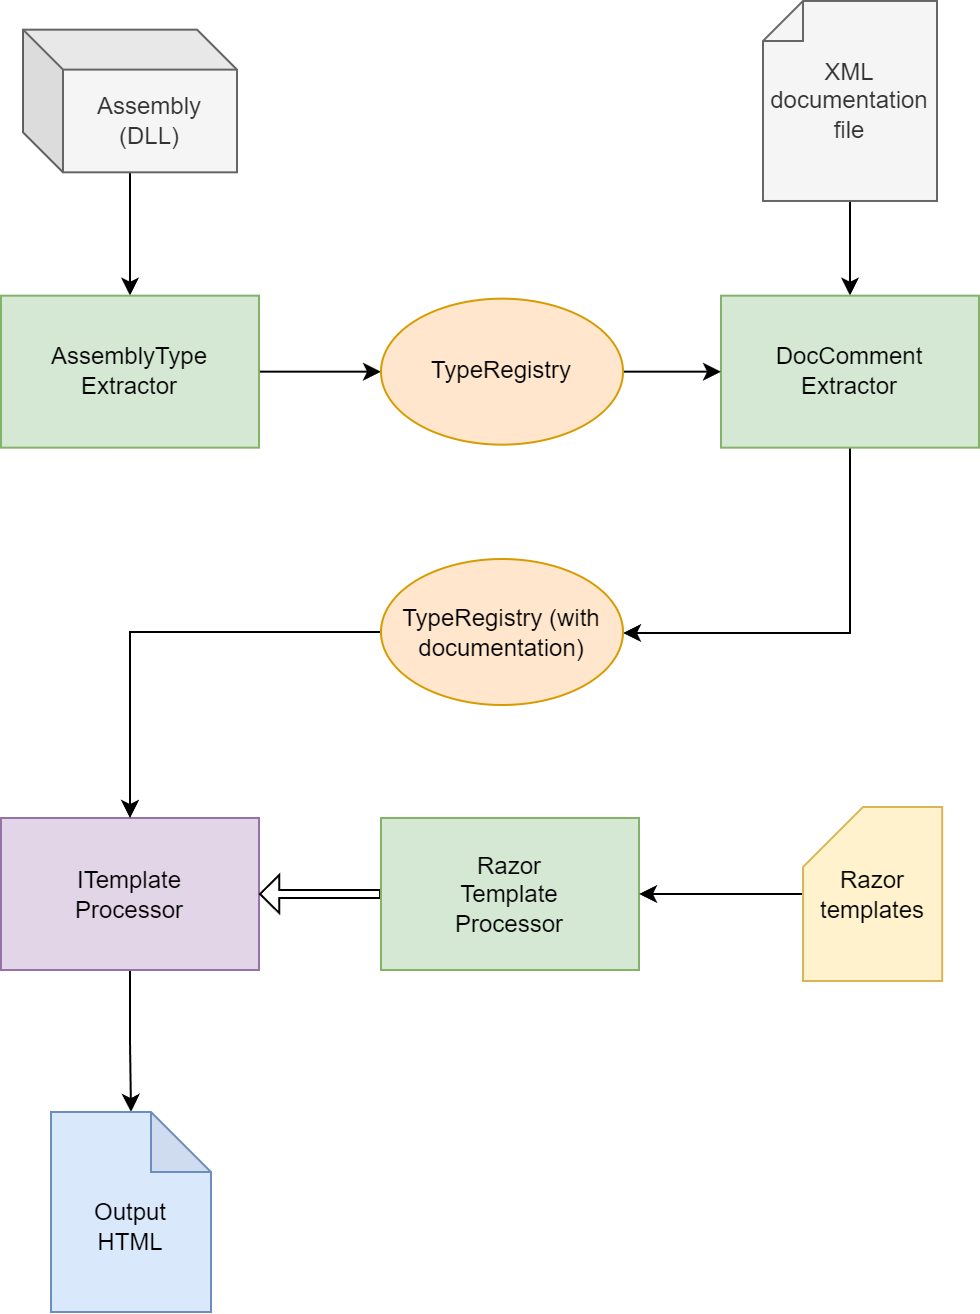
\includegraphics[width=1\linewidth]{img/workflow.png}
\caption{Program workflow}
\label{fig:workflow}
\end{figure}

\section{CodeElements}

This folder contains both type and member objects, introduced in sections~\ref{sec:member-repr} and \ref{sec:type-repr}.

\subsection{Members}

Member types and interfaces are stored in \texttt{Concrete/Members} and \texttt{Abstract/Members} subfolders.
First, there is a separate class for each kind of member, such as field, method, and property, as illustrated in Figure~\ref{fig:members-concrete}.
These classes have a suffix \textit{Data}, as opposed to the types provided by reflection, whose names end with \textit{Info}.
Thus, the types are named \texttt{FieldData}, \texttt{MethodData}, \texttt{PropertyData}, etc.
Also, we can notice there is a separate class for operators (\texttt{OperatorData}) and indexers (\texttt{IndexerData}), inherited from \texttt{MethodData}, or \texttt{PropertyData}, respectively.
That is because an overloaded operator in .NET is essentially a method using a special syntax, and similarly, an indexer is a special case of a .NET property.

The structure of member types has already been outlined in section~\ref{sec:member-repr}.
Basically, these types wrap the objects provided by reflection and provide all the necessary information about the member, as well as its documentation comments.
Additionally, there is a base class, called \texttt{MemberData}, containing the common properties, such as summary and remarks documentation, member name, ID string, etc.
Similarly, there is the \texttt{MethodLikeMemberData} class containing the functionality shared between methods and constructors.
Furthermore, the project also includes the \texttt{ParameterData} class representing a parameter.

It is worth noting that the properties representing documentation comments (such as \texttt{SummaryDocComment} or \texttt{RemarksDocComment}) are writable.
This is because the assignment of the documentation comments takes place after the members are loaded, as already explained in Figure~\ref{fig:workflow}.

Next, there are multiple interfaces representing members, whose hierarchy is displayed in Figure~\ref{fig:members-abstract}. 
First, there is a separate interface for each of the member types, called, e.g.
\texttt{IFieldData}, \texttt{IMethodData}, \texttt{IPropertyData}, etc.
Then, analogous to member classes, there are \texttt{IMemberData} and \texttt{IParameterData} interfaces.
Secondly, there are several super-interfaces that represent common properties of a selection of members.
TODO: rozepsat jednotlive interfaces?

The big difference between member interfaces and classes is that the interfaces provide a read-only view of the member data, because they are intended to be used by the template processors.
In contrast, the classes are intended to be used by the types performing the extraction and assignment of the documentation comments.

\begin{figure}[H]
\centering
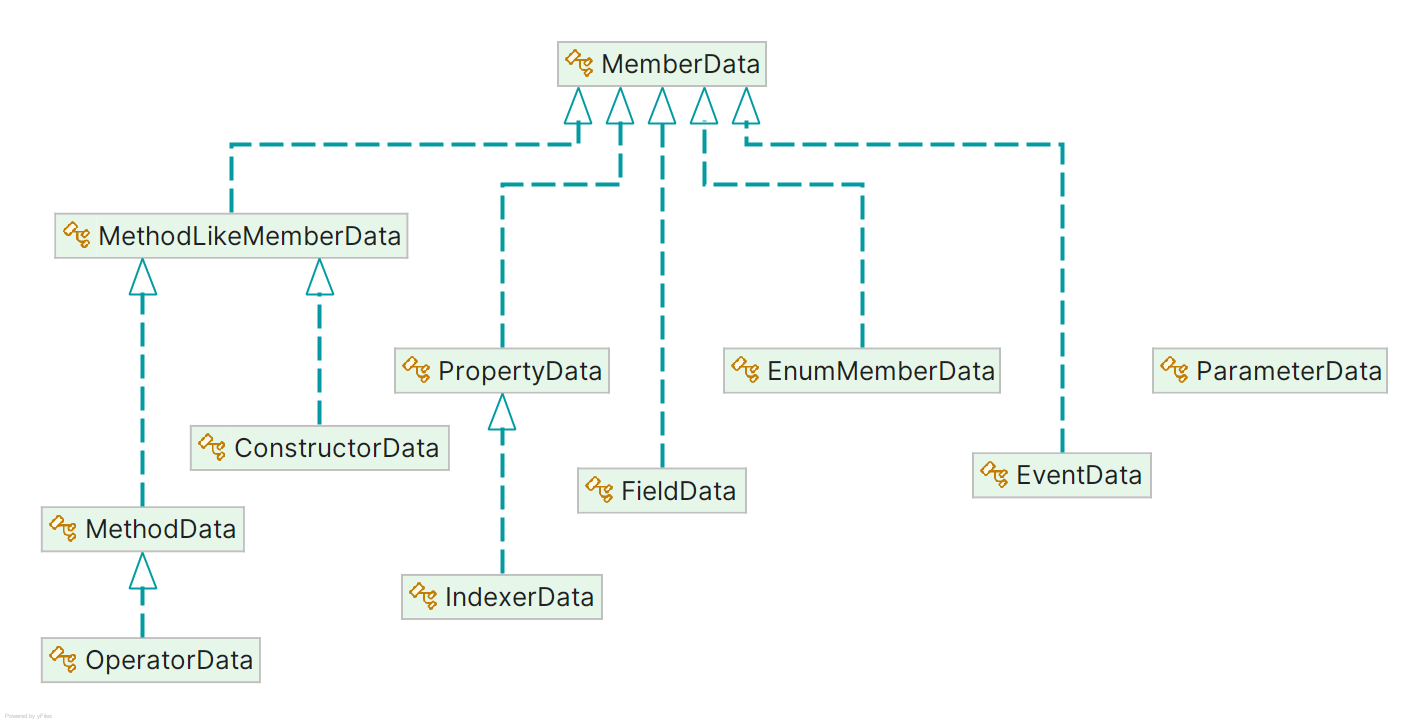
\includegraphics[width=1\linewidth]{img/diagram-members.png}
\caption{Member types -- inheritance graph}
\label{fig:members-concrete}
\end{figure}

\begin{figure}[H]
\centering
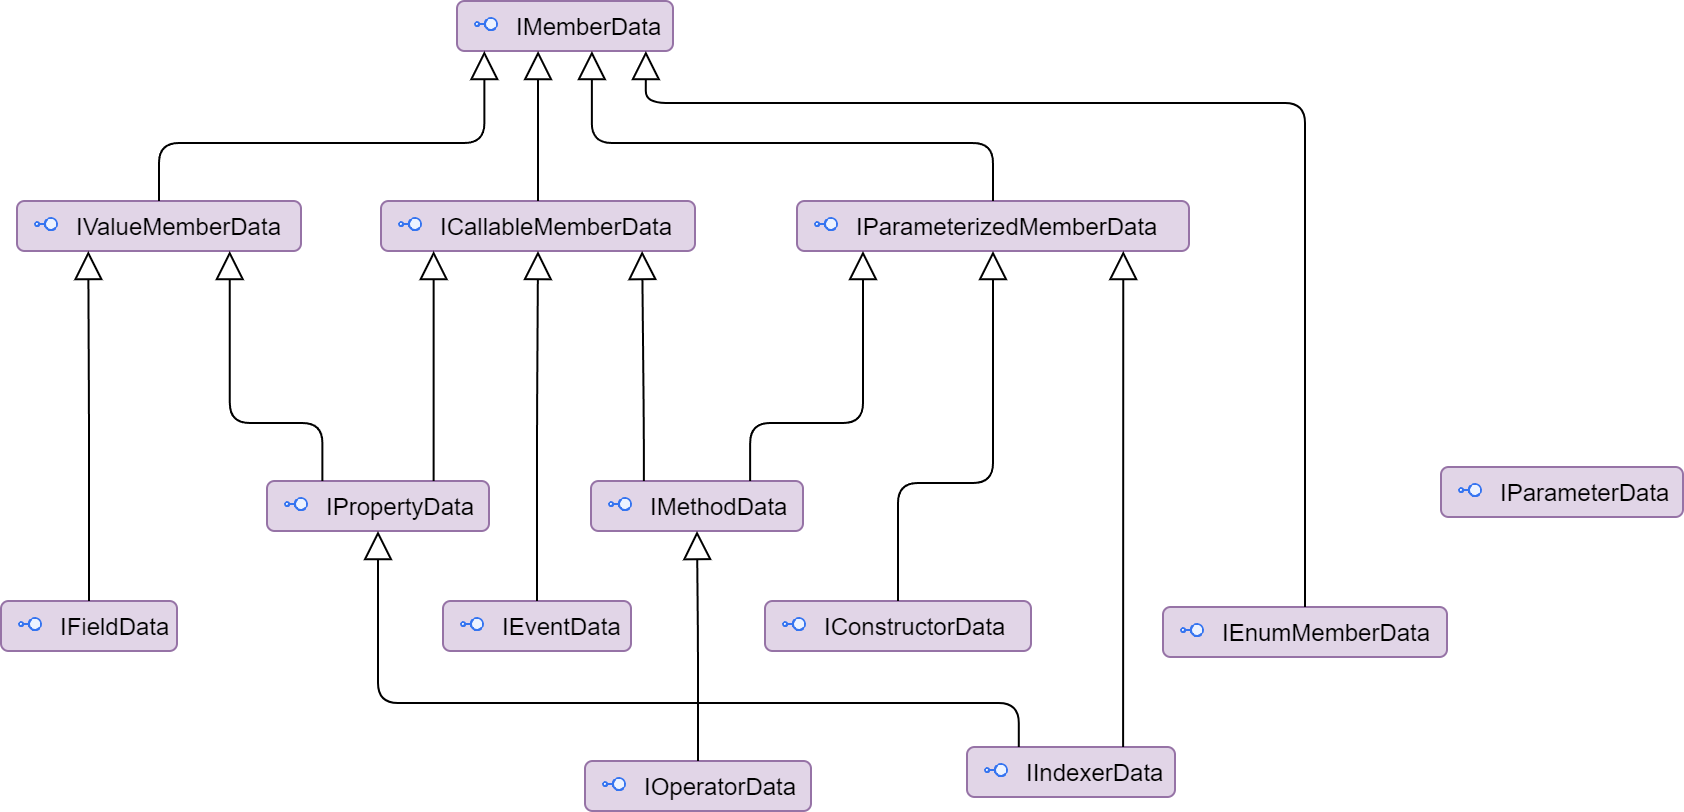
\includegraphics[width=1\linewidth]{img/diagram-member-interfaces.png}
\caption{Member interfaces -- inheritance graph}
\label{fig:members-abstract}
\end{figure}

\subsection{Types}
The objects representing types are stored inside the \texttt{Abstract/Types} and \texttt{Concrete/Types} folders.
Unlike the \texttt{System.Type} class, which covers all .NET types, there is a different class representing each kind of member:

\begin{itemize}
    \item \texttt{EnumData} -- represents enums.
    \item \texttt{DelegateData} -- represents delegates.
    \item \texttt{ObjectTypeData} -- represents other types (classes, structures, and interfaces).
\end{itemize}

All of these types inherit from the base class, called \texttt{TypeDeclaration}, which represents any type.



TODO: popsat strukturu

Furthermore, there is a TypeNameData class representing a field type or a return type.

Similarly, there are interfaces 

\subsection{Type registry}

All types are stored and passed in a type registry class, which contains all types,

\subsection{Tools}
TODO: vyhodit?

\section{Assembly Analysis}

This folder contains classes responsible for creating and populating the TypeRegistry with types extracted from an assembly.

Several classes: AssemblyTypeExtractor is the most important, as it extracts the data from an assembly in method XX.
There is a method for creating enum and delegate types.

For classes, interfaces and structs, the situation is quite different.
The construction of those is much more complicated, as they may contain various members.
For that reason, we used builder pattern, and created ObjectTypeBuilder class.
Moreover, each member object is created from the corresponding reflection type. 
This is done by creator classes, that are present for each member.
-> FieldDataCreator, MethodDataCreator, etc.

\section{Documentation Extraction}

\section{Template Generators}
\subsection{Template Model}
\subsection{Template Model Creators}
\subsection{Templates}

\section{Logging}
Describe what happens if there are errors.

\section{Tests}
Describe the packages used (xUnit, FluentAssertions, NSubstitute) and include snippets.

\subsection{Unit Tests}
\subsection{Integration Tests}

\section{Code Quality}

\subsection{.NET Analyzers}
\begin{itemize}
    \item Describe .NET analyzers.
\end{itemize}

\subsection{Code Style}
\begin{itemize}
    \item Describe code style.
\end{itemize}

\subsection{CI/CD}
\begin{itemize}
    \item Describe GitHub Actions.
\end{itemize}

\subsection{Workflow}
\begin{itemize}
    \item Feature branches, tasks, merge with linear history, etc.
\end{itemize}

\section{Extensibility}

\subsection{Custom Razor Templates}
Step-by-step guide.

\subsection{Custom Template Generator}
How to create a custom non-Razor template.

\chapter{User Documentation}

\section{How to Use}
Include screenshots of the result.

\section{Configuration}
\subsection{Option 1}
\subsection{Option 2}

\section{How to Make a Custom Razor Template}
